\chapter{Background} 
The aim of this work is to create a model that predicts if an article comment or a forum post can be classified as \emph{persuasive} or \emph{non-persuasive}. We'll first give general definitions about persuasion and argumentation, and how the corpus was annotated. Then, the tool that was used to perform the classification, DKPro Text Classification Framework, will be introduced and its functionalities will be explained.
\section{Argumentation} 
\subsection{General Definitions}
To better understand the vocabulary that will be used in this report, we give four important definitions:
\\
\\
\textbf{Debate} The process of inquiry and advocacy; the seeking of a reasoned judgement on a proposition. (\cite{freeley2000argumentation}, p. 2)
\\
\\
\textbf{Controversy} Controversy is an essential prerequisite of debate. Where there is no clash of ideas,
proposals, interests, or expressed positions on issues, there is no debate. (\cite{freeley2000argumentation}, p. 43)
\\
\\
\textbf{\Gls{argumentation}} Reason giving in communicative situations by people whose purpose is the justification of acts, beliefs, attitudes, and values. (\cite{freeley2000argumentation}, p. 2)
\\
\\
\textbf{\Gls{persuasion}} Communication intended to influence the acts, beliefs, attitudes, and values of others. (\cite{freeley2000argumentation}, p. 2)

\subsection{Persuasion}
Persuasion and argumentation are the essence of any debate about controversies. Whether on-line or face-to-face, people try to convince others about their opinions, values, and attitude towards that particular controversy using various kinds of argumentation.

Let’s assume a made-up example from a discussion forum about single-sex education, a quite
controversial topic. In one post, the author (i.e. \emph{Jack} ) writes:
\\
\\
\fbox{\begin{minipage}{1\textwidth}
\textbf{\#ex1 (forumpost, single-sex education)} I'm completely against single-sex education. This does not prepare students for real life where men and women live together!! –Jack
\end{minipage}}
\\

Jack’s intention here is not only to share his opinion but also to persuade other users in the
debate (and potentially all readers on the Internet). We can thus treat his message as persuasive
(also cf. definition above). The means he uses to persuade is argumentation, because he also gives
some reasons to support his stance towards the discussed topic.

However, the way people argue is not always as clear as in the example above. Suppose we have the following text from an actual debate about home-schooling:
\\
\fbox{\begin{minipage}{1\textwidth}
\textbf{\#203 (artcomment, homeschooling)} Teaching is not just subject knowledge (although
I’d be the last to downplay that). It is also meeting other people from all walks of life, dealing
with new situations, finding friends etc. I’ve always felt sorry for home-schooled kids. They
are being denied their childhood and adolescence by parents who want to exercise total power
of them, deny them the pains and pleasures that social experience brings. –JuniusPublicus
\end{minipage}}
\\

The author does not say explicitly that he/she is against home-schooling. However, he/she
provides some examples (necessity of social interaction, total power of parents) and expresses
feelings (sorry for home-schooled kids), so we can infer out the \emph{implicit} message. This example is
thus also \emph{persuasive} and \emph{argumentative}.
\subsection{Argumentation Mining}
With the emergence of information technologies and especially social media, the availability of argumentative textual data is always bigger. People tend to express their point of view and their feelings in article comments, on forum posts, blogging platforms, ect... As most of the data available online, they can be very messy and a lot of comments or posts are indeed off topic, forum spams\footnote{Forum spam consists of posts on Internet forums that contains related or unrelated advertisements, links to malicious websites, and abusive or otherwise unwanted information.} or \emph{trolls}\footnote{In Internet slang, a troll is a person who sows discord on the Internet by starting arguments or upsetting people, by posting inflammatory, extraneous, or off-topic messages in an online community (such as a newsgroup, forum, chat room, or blog) with the deliberate intent of provoking readers into an emotional response or of otherwise disrupting normal on-topic discussion.}. 
\
\begin{figure}[H]
    \centering
    \includegraphics[width=1\textwidth]{fig/spam.png}
    \caption[Short caption]{Example a the viagra spam in a forum}
    \label{fig:forumspam}
\end{figure}
\
Even so, it might be not trivial for some cases to judge if the author is completely off-topic or if he uses \emph{\gls{sarcasm}} or \emph{\gls{irony}} to support his opinion. One of the main step of \emph{Argumentation Mining}, as you can see on the dark grey rectangle of \ref{fig:argmining} is the detection of relevant documents, means the one that clearly show their argument but also the one which are persuasive but in an \emph{implicit} way.
\
\begin{figure}[H]
    \centering
    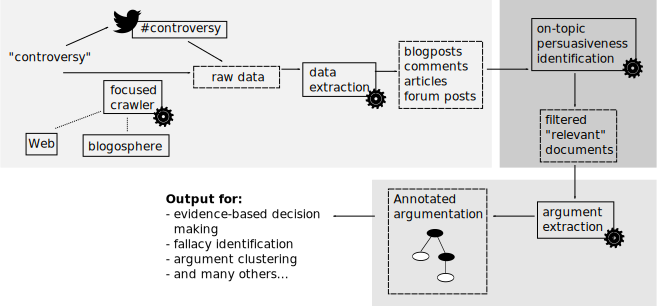
\includegraphics[width=1\textwidth]{fig/overview.png}
    \caption[Short caption]{The process of argumentation mining}
    \label{fig:argmining}
\end{figure}
\

\section{NLP and the DKPro Framework}
\subsection{Natural Language Processing}
Natural Language Processing or \emph{NLP} is a multidisciplinary field that combines Linguistics, Computer Science, Artificial Intelligence and its modern approach, \Gls{machine learning}.

NLP was actually the main goal of Computer Science's pioneers: write programs that would be able to understand human speech as it is written and spoken. This Fantasy which is becoming more and more true gives the actual definition of NLP:  ability of a computer program to understand humans natural language. 

The development of NLP applications is challenging since computers and programming languages are highly structured contrary to human language which is not always precise. A lot of misunderstands come from ambiguities in intonation, context (a certain sentence can be serious or sarcastic in different contexts), the social background or the dialect used. Even so, a lot of progress have been made, and here is a non-exhaustive list of fields that emerged from NLP:
\begin{itemize}
  \item Sentence segmentation, part-of-speech tagging and parsing.  
  \item Speech Recognition
  \item Automated Translation
  \item Automatic Summaries
\end{itemize}

In this work, we'll see how NLP can help us in Argumentation Mining and Persuasiveness detection. 
 
\subsection{UIMA}
DKPro stands for \emph{Darmstadt Knowledge Processing}
\cite{GurevychEtal2007dkpro0} and it's a software suite for NLP based on the Apache UIMA Framework. UIMA are software systems that analyse large volumes of unstructured information in order to discover knowledge that is relevant to an end user. An example UIMA application might ingest plain text and identify entities, such as persons, places, organizations; or relations, such as works-for or located-at:

\
\begin{figure}[H]
    \centering
    \includegraphics[width=1\textwidth]{fig/uima.png}
    \caption[Short caption]{UIMA: Order unstructured data, from UIMA website \cite{uima:Online}}
    \label{fig:uima}
\end{figure}
\

The real power of UIMA is its Analysis Engines (AE) which basically analyse a document and record descriptive attributes. Those descriptive attributes will form the document's metadata that will be used for further analysis (such as Text Classification in our case).

\subsection{DKPro Core}
Many NLP tools are already freely available in the NLP research community. DKPro Core \cite{TUD-CS-2014-0864} provides UIMA components wrapping these tools so they can be used interchangeably in UIMA processing pipelines. The provided components wrap a constantly growing set of stand-of-the-art NLP tools and also include several original components written Java covering a wide range of tasks including: \gls{tokenization}/segmentation, compound splitting, stemming, \gls{parts-of-speech} tagging, lemmatization, constituency parsing, dependency parsing, named entity recognition, coreference resolution, language identification, spelling correction, grammar checking, and support for reading and writing various file and corpus formats. 
\
\begin{figure}[H]
    \centering
    \includegraphics[width=1\textwidth]{fig/dkpro-pipeline.png}
    \caption[Short caption]{DKPro Core Pipeline}
    \label{fig:dkpro-pipeline}
\end{figure}
\
Core has several annotators either developed in-house or wrapped\footnote{A wrapper function is a subroutine in a software library or a computer program whose main purpose is to call a second subroutine or a system call with little or no additional computation. Source: Wikipedia} from the state-of-the-art NLP libraries. Here is a non exhaustive list:
\begin{itemize}
  \item \textbf{Stanford NLP} - segmentation, la lemmatisation, part of speech...
  \item \textbf{OpenNLP} - machine learning based toolkit for the processing of natural language text: tokenization, sentence segmentation, part-of-speech tagging, named entity extraction, chunking, parsing, and coreference resolution. 
  \item \textbf{CleanNLP} - robust NLP components implemented in Java for part-of-speech tagging, dependency parsing, semantic role labelling... 
\end{itemize}

\subsection{DKPro Text Classification}
The aim of DKPro TC (commonly called TC) is to allow the user to apply machine learning algorithms easily on the extracted annotations. This framework was built in order to execute the following tasks:
\begin{itemize}
  \item \Gls{supervised learning} Classification. The user should provide annotated textual data.
  \item Can work atomically on text (word, sentence, paragraph) or on pairs of documents.
  \item Can perform \gls{single-label} classification, \gls{multi-label} classification and \gls{regression}.
\end{itemize}

Concerning the algorithms used, TC relies on Weka\footnote{http://www.cs.waikato.ac.nz/ml/weka/} (\textit{Waikato Environment for Knowledge Analysis}). Developed by the Waikato University in New Zealand, Weka is an open-source Data Mining software written in Java, which makes available to its users not only Machine Learning algorithms but also processing features (attribute selections and transformations) and a user interface with visualization tools. Regularly updated, Weka is one of the main state-of-the-art data mining software used in research. 
\

Weka communicates with TC thank to one major component: the \textbf{feature}. In the code, the feature is usually a class that computes a certain value (ex: length of a post, number of adjectives in a text, ect...) using the annotation provided by the DKPro pipeline. Features can be implemented by polymorphism from the mother-class \textit{FeatureExtractorResource$\_$ImplBase}. The results are then saved in an \textit{ARFF} \footnote{An ARFF (Attribute-Relation File Format) file is an ASCII text file that describes a list of instances sharing a set of attributes.} file, which corresponds to Weka's format files.  
\
\begin{figure}[H]
    \centering
    \includegraphics[width=1\textwidth]{fig/TC-modes.png}
    \caption[Short caption]{The different usages of DKPro TC}
    \label{fig:dkpro-tc-usages}
\end{figure}
\

In a nutshell, TC adds 4 more steps to DKPro Core:
  \begin{itemize}
  \item A step where the data are labelled, since we're doing supervised learning. 
  \item Extraction of the features from the annotations.
  \item Data Processing and Cross Validation (\cref{sec:bincla})
  \item Report of the results (Accuracy, Macro F-Measure, ect...)
\end{itemize}  

The TC developers give regularly some helpful tutorials on their website\footnote{https://code.google.com/p/dkpro-tc/wiki/DemoExperiments}. 
\
\vspace{0.2cm}
\\
\textbf{License and usage}

While most DKPro TC modules are available under the Apache Software License (ASL) version 2, there are a few modules that depend on external libraries and are thus licensed under the General Public Licence (GPL). 
\\
The SVN\footnote{Apache Subversion (often abbreviated SVN, after the command name svn) is a software versioning and revision control system distributed as free software under the Apache License.} commits of the different modules are available through Google code and the integration of new functionalities in a project is made possible by Maven\footnote{Apache Maven is a software project management and comprehension tool. Based on the concept of a project object model (POM), Maven can manage a project's build, reporting and documentation from a central piece of information.}. It's also possible to use DKPro TC with Groovy which is an object-oriented programming language for the Java platform and destined to be run on a server. 

















